\documentclass{article}
\usepackage[utf8]{inputenc}
\usepackage{multicol}
\usepackage{geometry}
\usepackage{amsmath}
\usepackage{graphicx}
\usepackage{subcaption}
\usepackage{float}
\geometry{
    left=25mm,
    right=25mm,
    top=27mm,
    bottom=27mm
}

\title{TWA + Rydberg Facilitation HiWi}
\author{Hoang Nguyen}
\date{\today}

\begin{document}

\maketitle

    \section{Single Driven Atom}
    In this section, I explore the dynamics of a single atom driven by an external field. I provide both exact solutions using quantum mechanical methods and approximate methods via the Truncated Wigner Approximation (TWA). This section serves as the foundation for understanding how external driving impacts atomic dynamics, which I will extend later to many-atom systems.

    \subsection{Direct calculation of driven single atom}
    The direct calculation method involves solving the quantum evolution of a single atom's density matrix under the influence of driving fields. I use the density matrix formalism to track population and coherence between atomic levels.
    
    \subsubsection{Expectation value of $\hat{S_z}$}
    The expectation value of the collective spin component $\hat{S}_z$ is calculated using the density matrix $\rho$:
    \begin{equation}
        \langle \hat{S}_z \rangle = \operatorname{Tr}\left\{\hat{S}_z \rho\right\}
    \end{equation}
    This provides insight into the population difference between energy states as a function of time.

    \subsubsection{Maxwell-Bloch Equation}
    The Maxwell-Bloch equations describe the time evolution of the atom's density matrix elements. The system evolves based on decay rate $\Gamma$, Rabi frequency $\Omega$, and detuning $\Delta$. These equations provide an exact quantum mechanical description of the atom's dynamics:
    \begin{equation}
        \dot{\rho}_{gg} = -\Gamma \rho_{ee} + i \Omega (\rho_{ge} - \rho_{eg})
    \end{equation}
    
    \begin{equation}
        \dot{\rho}_{ge} = \left(i \Delta - \frac{\Gamma}{2}\right) \rho_{ge} + i \Omega (\rho_{ee} - \rho_{gg})
    \end{equation}
    
    \begin{equation}
        \dot{\rho}_{eg} = -\dot{\rho}_{ge}
    \end{equation}
    
    \begin{equation}
        \dot{\rho}_{ee} = -\dot{\rho}_{gg}
    \end{equation}
    These equations track the population dynamics of ground and excited states, along with the coherences between them.

    \subsection{TWA for single driven atom}
    The Truncated Wigner Approximation (TWA) simplifies the quantum mechanical system by approximating it using classical trajectories with stochastic noise. We convert the exact quantum equations into stochastic differential equations (SDEs) using the Itô formalism. Here, the drift and diffusion terms represent the deterministic evolution and the quantum noise, respectively.

    Ito SDEs:
    \subsubsection{Drift term}
    The drift term defines the deterministic evolution of the system, based on the Rabi frequency and detuning:
    \begin{equation}
        d\theta = \Gamma_0 \left( \cot \theta + \frac{\csc \theta}{\sqrt{3}} \right) dt, \tag{16a}
    \end{equation}
    \begin{equation}
        \frac{d\phi}{dt} = 2 \Omega \cot(\theta) \cos(\phi) - \Delta
    \end{equation}
    
    \subsubsection{Diffusion term}
    The diffusion term introduces noise due to quantum fluctuations:
    \begin{equation}
        d\phi = \sqrt{\Gamma_0 \left( 1 + 2 \cot^2 \theta + \frac{2 \cot \theta \csc \theta}{\sqrt{3}} \right)} dW_\phi, \tag{16b}
    \end{equation}
    
    The following figure shows the comparison between the exact solution and the TWA approximation for the dynamics of a single driven atom:
    \begin{figure}[H]
        \centering
        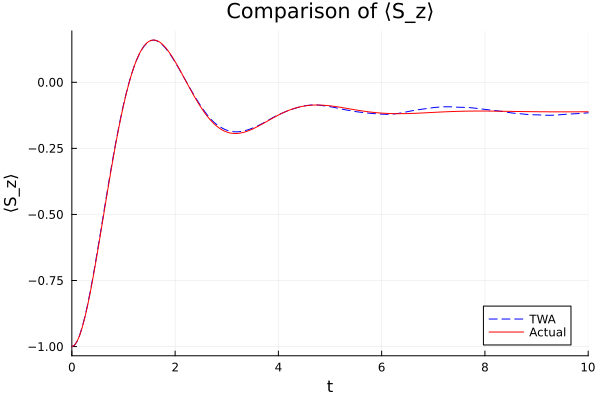
\includegraphics[width=0.65\linewidth]{Sz.png}
    \end{figure}
    
    The simulation models the dynamics of a driven single atom and compares the Maxwell-Bloch equations and TWA (Itô SDEs). The Maxwell-Bloch equations provide the exact quantum solution, while TWA approximates the dynamics by incorporating stochastic noise, which captures quantum fluctuations. The comparison helps assess the accuracy and computational cost of TWA in simulating quantum systems.
    
    \section{Dicke Superradiance}
    In this section, I extend my analysis from a single atom to a system of many atoms. The Dicke model describes superradiant emission from a collection of atoms. We will calculate key observables, including the collective spin component $\hat{S}_z$ and the radiated intensity, using both direct quantum calculations and TWA.

    \subsection{Direct calculation for Dicke}
    In the Dicke model, we use the density matrix to compute the collective spin dynamics and radiated intensity from a large ensemble of atoms.

    \subsubsection{Expectation value of $\hat{S_z}$}
    We calculate the expectation value of the collective spin component $\hat{S}_z$ using the trace over the density matrix $\rho$:
    \begin{equation}
        \langle \hat{S}_z \rangle = \operatorname{Tr}\left\{\hat{S}_z \rho\right\}
    \end{equation}
    
    Using the ansatz for the Dicke states:
    \begin{equation}
        \hat{\rho} = \sum_{m=-N/2}^{N/2} \rho_m |j, m\rangle \langle j, m| \tag{2.29}
    \end{equation}

    \begin{equation}
        \hat{S}_z |j, m\rangle = m |j, m\rangle
    \end{equation}
    
    The final expression for the expectation value:
    \begin{equation}
        \langle \hat{S}_z \rangle = \sum_{m=-N/2}^{N/2} \rho_m m
    \end{equation}
    This gives the average spin component along the z-axis for the ensemble.

    \subsubsection{Solve $\langle \hat{S_z} \rangle$ with ODE of $\rho_m$}
    To solve the dynamics of $\rho_m$, we use the following system of differential equations:
    \begin{equation}
        \begin{aligned}
            \frac{d}{dt} \rho_m &= -\Gamma_0 (j + m)(j - m + 1)\rho_m \\ 
            &\quad + \Gamma_0 (j + m + 1)(j - m)\rho_{m+1} \\ 
            &= \Gamma_0 [g(j, m + 1)\rho_{m+1} - g(j, m)\rho_m],
        \end{aligned} \tag{2.30}
    \end{equation}
    
    \subsubsection{Radiated intensity}
    The radiated intensity is derived from the time derivative of the expectation value of $\hat{S}_z$:
    \begin{equation}
        \gamma(t) = -\frac{d}{dt}\langle\hat{S}^{z}\rangle = \Gamma_{0}\int_{-j}^{j}dm~g(m)\rho(m,t) \\
        = \Gamma_{0}N^{2}f(Ne^{-\Gamma_{0}t}).
    \end{equation}

    \subsection{TWA for Dicke}
    For the Dicke model, the TWA approach approximates the quantum system using stochastic trajectories for each atom. We derive the drift and diffusion terms for the SDEs governing the dynamics of each atom.

    \subsubsection{Diffusion and drift terms}
    The drift and diffusion terms for the atomic angles $\theta_n$ and $\phi_n$ are:
    \begin{align}
        d\theta_n &= \left[\frac{\Gamma_{mn}}{2}\cot\theta_n + \sqrt{3}\sum_{m=1}^{N}\sin\theta_m \left(J_{mn}\sin\phi_{mn} + \frac{\Gamma_{mn}}{2}\cos\phi_{mn}\right)\right] dt \nonumber \\
        &\quad + \sum_{m=1}^{N} G_{nm} \left(-\cos\phi_n dW_{\theta m} + \sin\phi_n dW_{\phi m}\right), \\
        d\phi_n &= \sqrt{3}\cot\theta_n \sum_{m=1}^{N}\sin\theta_m \left(-J_{mn}\cos\phi_{mn} + \frac{\Gamma_{mn}}{2}\sin\phi_{mn}\right) dt \nonumber \\
        &\quad + \sum_{m=1}^{N} G_{nm} \cot\theta_n \left(\sin\phi_n dW_{\theta m} + \cos\phi_n dW_{\phi m}\right).
    \end{align}

    The following figures show the comparison between the TWA and direct simulations for both the expectation value of $\hat{S}_z$ and the radiated intensity:
    \begin{figure}[H]
        \centering
        \begin{subfigure}{0.45\textwidth}
            \centering
            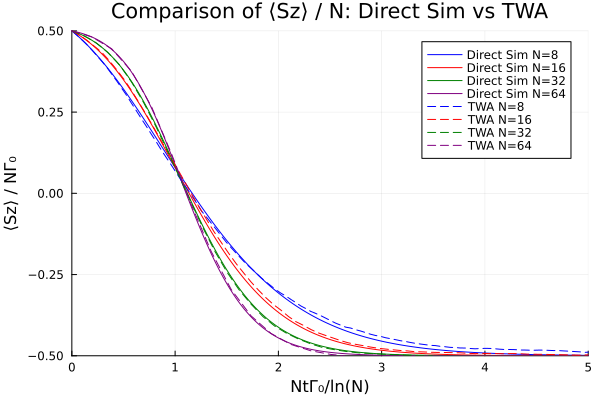
\includegraphics[width=\linewidth]{TWA_direct_Sz.png}
            \caption{Comparison of $\langle \hat{S}_z \rangle$}
            \label{fig:subfig1}
        \end{subfigure}
        \hfill
        \begin{subfigure}{0.45\textwidth}
            \centering
            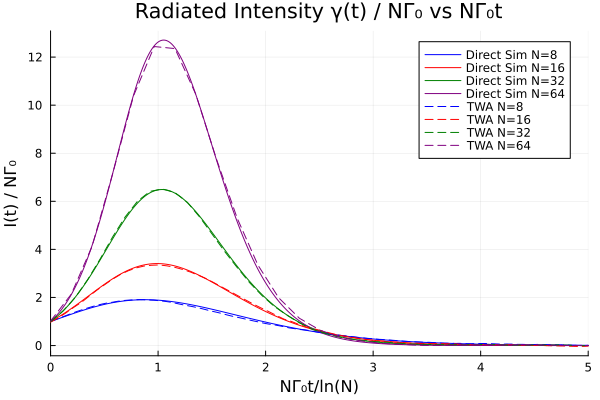
\includegraphics[width=\linewidth]{intensity.png}
            \caption{Comparison of radiated intensity}
            \label{fig:subfig2}
        \end{subfigure}
        \caption{Comparison between TWA and direct simulations for Dicke model}
        \label{fig:overall}
    \end{figure}

    \subsubsection{Additional relations and final intensity expression}
    The following equation relates the collective spin operator $\hat{S}$ to its components:
    \begin{equation}
        \hat{S}(\{c_n\})^\dagger \hat{S}(\{c_n\}) \leftrightarrow |S^-(\{c_n\})|^2 + \frac{1}{2} S^z(\{ |c_n|^2 \})
    \end{equation}

    Finally, the expression for the radiated intensity as a function of time is given by:
    \begin{equation}
        I(t) = - \frac{\sqrt{3}}{2} \Gamma_0 \sum_n \cos \theta_n - \frac{3}{4} \sum_{mn} \Gamma_{mn} \sin \theta_m \sin \theta_n \cos(\phi_m - \phi_n)
    \end{equation}

    The Truncated Wigner Approximation (TWA) is a semiclassical approach used to simulate quantum many-body systems like the Dicke model. It approximates quantum dynamics by evolving classical trajectories in phase space, providing computational efficiency. Comparisons between TWA and direct quantum simulations for $S_z$ and intensity show that results largely agree, though minor discrepancies arise due to the approximations in TWA. 

\end{document}
